\chapter{About this project}\label{ch:about}


This project is part of a bachelor-thesis in engineering sciences [ELO-ICT].
The main purpose of this thesis is to map the sound intensity or sound pollution from different areas into an application. 

The numerous nodes will capture sound. Then because we are using LoRa we can't send too much data it is important that the processing is done by the nodes. Finally the nodes will send what they calculated to the gateway which in turn will send it to the cloud. 

From the cloud the data can be pulled and displayed in a visual manner onto the application.

\begin{figure}[hb]\centering
     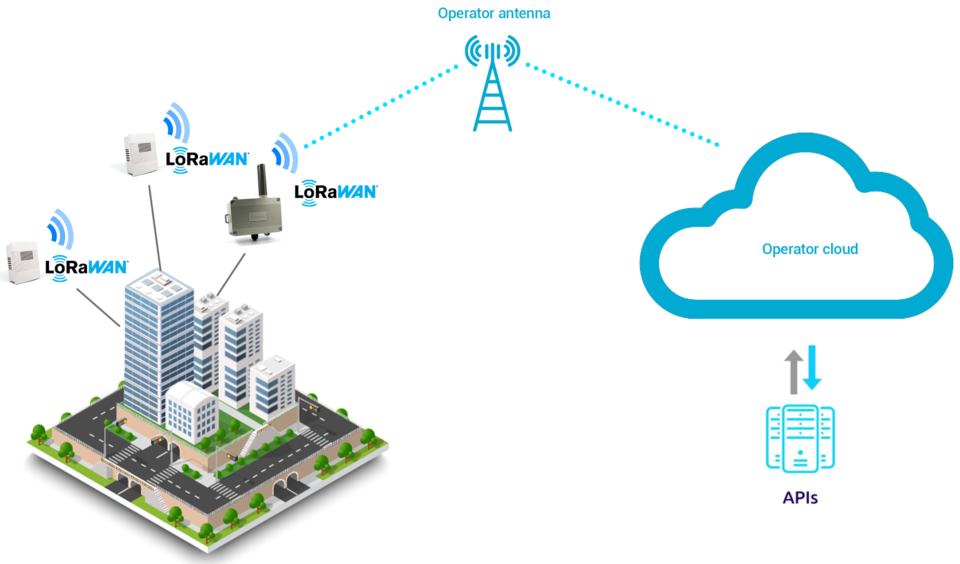
\includegraphics[width=1\textwidth,height=1\textheight,keepaspectratio]{figs/IOT_Netwerk}
	\caption{Visual representation of our project}\label{fig:radiation}
\end{figure}

Different kinds of technologies will be used in this project.
\begin{itemize}
    \item KiCad to design our embedded-systems [Nodes]
    \item LoRa and IP for data transmission
    \item MicroPython to program the embedded-systems
    \item a Linux VM as our network- and application server
\end{itemize}

 





